% !Mode:: "TeX:UTF-8"
% !TEX root = ..\Literature_Translation.tex
\kchapter{阶段建模}
\ksection{阶段1}
阶段1的目标是找到只有1个装配夹具,而不顾可用工人数时的最大生产能力,即工人数量无限的情况下最小化制造期。
接下来的模型是基于Coffman(1976), Baker(1974), Morton和 Pentico(1993), Leung(2004)和 Pinedo(2008), Potts和 Strusevich(2009)的作业车间调度问题。设$L$为任务数,对于每个任务$j=1,2,...,J$:\\[3pt]
\indent$p_j:$ 任务$j$在装配夹具的操作持续时间\\
\indent$q_j:$ 任务$j$在工作台的操作持续时间

此外,需要对每个任务对$(j,k),j\neq k$定义集合如下:
\begin{numcases}{}
A = \left\{(j,k)\mid\text{任务$j$需在任务$k$开始前结束}\right\}\notag\\
B = \left\{(j,k)\mid\text{任务$j$和任务$k$在夹具内的邻接工作台操作}\right\}\notag\\
C = \left\{(j,k)\mid\text{任务$j$和任务$k$在夹具内同一个位置操作}\right\}\notag
\end{numcases}

决策变量建模如下:
\vspace{-3pt}
\begin{numcases}{y_{jk} = }
1\qquad\text{如果任务$j$在任务$k$前调度}\notag\\
0\qquad\text{其他情况}\notag 
\end{numcases}

$t_j:$ 任务$j$的开始时间

$t_F:$ 制造期

那么阶段1的数学模型如下:
\begin{align}
&\label{equb:1} \min \quad t_f \\
&\label{equb:2} t_j + p_j + q_j \leqslant t_F \qquad j = 1,...,J\\
&\label{equb:3} t_k + M(1 - y_{jk}) \geqslant t_j + p_j \qquad \text{对于所有} (j,k)\in C\\
&\label{equb:4} t_j + M\times y_{jk} \geqslant t_k + p_k \qquad \text{对于所有} (j,k)\in C\\
&\label{equb:5} t_k \geqslant t_j + p_j + q_j  \qquad \text{对于所有} (j,k)\in A\\
&\label{equb:6} t_k + M(1 - y_{jk}) \geqslant t_j + p_j \qquad \text{对于所有} (j,k)\in B\\
&\label{equb:7} t_j + M\times y_{jk} \geqslant t_k + p_k \qquad \text{对于所有} (j,k)\in B\\
&\label{equb:8} t_j \geqslant 0,\ y_{jk}\in \{0,1\},\quad j=1,...,J,\quad k=1,...,J,\quad j\neq k
\end{align}

在模型(\ref{equb:1}) -- (\ref{equb:8})中,目标函数\eqref{equb:1}最小化了制造期$t_F$,约束\eqref{equb:2}保证了制造期要不小于任何调度内任务的完成时间。
约束\eqref{equb:3}和(\ref{equb:4})避免了在同个装配工作站的任务重叠,需要注意的是,这两约束只为同工作站装配任务对$j$和$k$定义。
也需注意的是约束\eqref{equb:3}和(\ref{equb:4})是相互分离的,即一个激活时,另一个是冗余的,反之亦然(William,1999)。
参数M 是一个足够大的正数,可以定义为:$\sum_{j=1}^J(p_j + q_j)$。
约束\eqref{equb:5}保证先后之间的关系。
约束\eqref{equb:6}和(\ref{equb:7})保证需要用到邻接工作站的任务不会同时被调度。
约束\eqref{equb:8}参考决策变量的定义域。

以防万一,包括一些任务可能在0时刻之后提交,并且有些任务可能有工期(即防止任务与多于1架飞机有关而产生不同的工期),我们可以定义:\\[3pt]
\indent $r_j:$ 任务$j$的提交日期

$d_j:$ 任务$j$的工期\\
这样一来上述模型可以简单地改变以包含下述约束:
\begin{align}
&\label{equb:9} t_j \geqslant r_j \qquad \text{对于一些$j$}\\
&\label{equb:10} t_j + p_j + q_j \leqslant d_j \qquad \text{对于一些$j$}
\end{align}
其中,\eqref{equb:9}保证每一个任务$j$都在其提交日期$r_j$之后才被调度,\eqref{equb:10}保证每个任务$j$都在工期$d_j$前完成。
同时注意参数M 需要相应修改以使提交日期$r_j$非空。

\ksection{阶段2}
在本阶段,要考虑2个装配队伍:夹具装配队伍和工作台队伍。
该阶段的目标是最小化总成本或人工数量,并且在给定工期前完成。
在一些变化后,该问题可以建模成考虑时间因素的项目调度问题。
这个项目包含多个活动,每个活动都需要1种以上的资源使其得以执行。
通常,活动有其已知的持续时间,并且由于技术限制,它们中间往往存在先后关系。
本文研究的项目调度问题考虑有限但可再生资源,即被使用过后,该资源可以再次被使用(员工、机器设备等都是可再生资源的例子)。
其目标是在最小化资源使用量,考虑活动的先后关系,可用资源量,以及在给定工期的前提下,找到一个可行调度。
在项目调度的范畴中,该问题以时间约束的项目调度闻名(Brucker, Drexl, Mohring, Neumann,和Pesch, 1999; Yamashita和 Morabito, 2009)。
回顾项目调度问题可见Brucker等(1999), Hartmann和 Kolisch(2000), Kolisch和 Padman(2001), Guldemond, Hurink, Paulus,和 Schutten(2008)的文章。

将项目调度问题和本文研究的邻接约束调度问题相互对应并不困难,可将每个装配操作对应成活动,这样的话操作的时间(在夹具或工作台中)对应成活动的持续时间,操作所遵守的顺序(见\reff{fig:subsetoperation})对应活动的先后关系。
阶段1模型将2个操作对应1个任务,与之不同的是阶段2模型中1个操作对应1个活动。该模型需要10种类型的资源:
\begin{asparaenum}[(a)]
\item 夹具中的工人;
\item 工作台上的工人;
\item 8个夹具中各自的工作站。
\end{asparaenum}

在本阶段,在夹具和在工作台的工人数量可得。另一方面,对应于需要用到的工作站数量的资源类型是本问题的参数。
为了在该模型中正确描述邻接约束,可以人工假设每个对应到夹具工作站的资源类型用有2个可用单元,并且在这些夹具上处理的活动需要从工作站上获取2个资源,加上相邻两工作站间的1个资源。
\begin{figure}[h]
\centering\caption{装配夹具的工作站使用和资源的表示\label{fig:representationofresourcesandworkstations}}
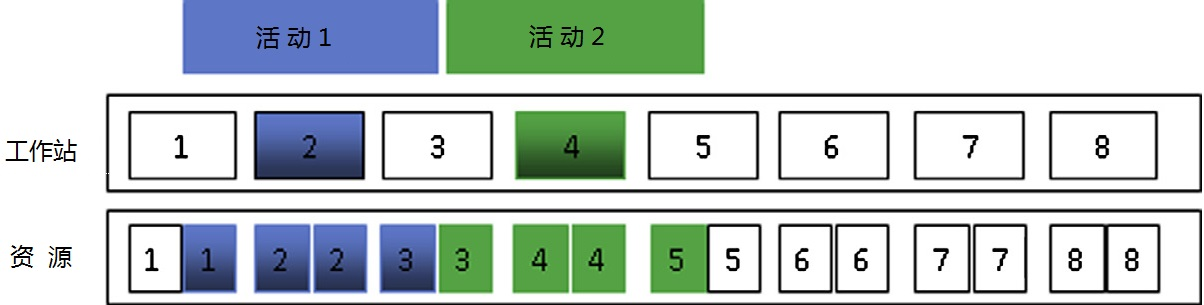
\includegraphics[width=12cm]{resourceandworkstation}
\end{figure}
\reff{fig:representationofresourcesandworkstations}举了一个例子,其中活动1在工作站2进行装配,它占用了2个工作站2的资源,其中1个是来自邻接工作站1,另一个来自邻接工作站3。
类似的,活动2占用2个工作站4的资源,其中1个来自邻接工作站3,另一个来自邻接工作站5。
因此,工作站1,3,5将被邻接约束所阻塞,不能和工作站2,4同时工作。
然而,任何使用工作站6,7,8的活动可以在处理活动1,2时同时进行。